\documentclass{beamer}
\usepackage[T1]{fontenc} \usepackage{lmodern} \usepackage[utf8]{inputenc}
\usepackage[english]{babel} \usepackage{booktabs}
\usepackage{graphicx,subcaption} \usepackage{amssymb,amsmath}
\graphicspath{{img/}}
\usepackage[citestyle=authoryear,bibstyle=authoryear,backend=biber,url=false,doi=false,isbn=false]{biblatex} \bibliography{refs}
\usepackage{hyperref} \hypersetup{
	pdfauthor={Michaël Defferrard},
	pdftitle={Final project},
	pdfsubject={Data Science}
}

% Make Adobe Reader use the RGB rendering model for pages with transparency.
\pdfpageattr{/Group << /S /Transparency /I true /CS /DeviceRGB>>}

\mode<presentation>{
	\usetheme{Malmoe}
	\usecolortheme{beaver}
	\setbeamertemplate{footline}[page number]
	\setbeamertemplate{navigation symbols}{}
}

%------------------------------------------------

\DeclareMathOperator*{\diag}{diag}
\DeclareMathOperator*{\argmin}{arg\,min}
\DeclareMathOperator*{\spn}{span}
\newcommand{\G}{\mathcal{G}}
\newcommand{\V}{\mathcal{V}}
\newcommand{\E}{\mathcal{E}}
\newcommand{\bO}{\mathcal{O}}
\newcommand{\R}{\mathbb{R}}

\newcommand{\good}[1]{{\color[rgb]{0.2,0.6,0.2}#1}}
\newcommand{\bad}[1]{{\color{red}#1}}
\newcommand{\txt}[1]{\hspace{.5cm} \text{#1} \hspace{.5cm}}
\newcommand{\define}[1]{\item{\usebeamercolor[fg]{enumerate item}#1}:}
\newcommand{\HRule}{{\usebeamercolor[bg]{subsection in head/foot} \rule{\linewidth}{0.5mm}}}

%------------------------------------------------

\begin{document}

\begin{frame}[plain]
	%\titlepage
	\begin{center}

		\small A Network Tour of\\
		\vspace{0.2cm}
		\textsc{\large Data Science}\\
		\vspace{0.7cm}

		\HRule
		\vspace{0.65cm}
		{
			\usebeamercolor[fg]{frametitle}
			\textsc{\Large Final Project}\\
			\vspace{0.2cm}
		}
		\HRule
		\vspace{1.0cm}

		\begin{minipage}{0.32\textwidth}
			\begin{center} \footnotesize
				Michaël \textsc{Defferrard}
			\end{center}
		\end{minipage}
		\begin{minipage}{0.32\textwidth}
			\begin{center} \footnotesize
				Xavier \textsc{Bresson}
			\end{center}
		\end{minipage}
		\begin{minipage}{0.32\textwidth}
			\begin{center} \footnotesize
				Pierre \textsc{Vandergheynst}
			\end{center}
		\end{minipage}

		\vspace{1.0cm}
		\footnotesize EPFL LTS2 Laboratory\\
		\vspace{0.1cm}
		\footnotesize November 14, 2016

	\end{center}
\end{frame}

%------------------------------------------------

\begin{frame}
	\frametitle{Data Scientist}
	\begin{figure}
		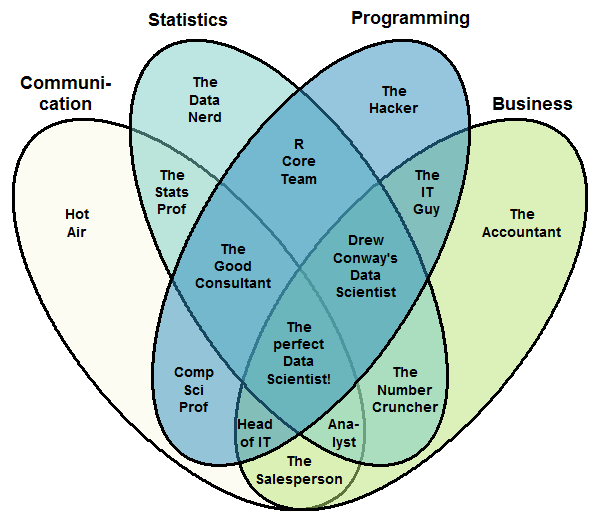
\includegraphics[height=0.8\textheight]{data_scientist}
	\end{figure}
\end{frame}

%------------------------------------------------

\begin{frame}
	\frametitle{Project}
	\begin{enumerate}
		\item Define a problem.
		\vfill
		\item Solve it in a Jupyter notebook using the Data Science process.
		\vfill
		\item Handle your solution for grading.
	\end{enumerate}
\end{frame}

%------------------------------------------------

\begin{frame}
	\frametitle{Problem}
	\begin{center}
		Find a problem you want to solve.
	\end{center}
	\vfill
	%Sources of inspiration:
	\begin{itemize}
		\item Classic problems: Computer Vision, Natural Language Processing.
		\vfill
		\item Social websites are a wealth of information.\footnote{Not only
			Facebook and Twitter, but also GitHub, Pinterest, StackOverflow,
			YouTube, LinkedIn, Instagram, Tumblr, etc.}
		\vfill
		\item Your own interests: scientific, hobbies or otherwise.
		\vfill
		\item Open challenges, e.g. \href{https://www.kaggle.com/}{kaggle}.
		\vfill
		\item Any other.
		\vfill
		\item Discuss with us!
	\end{itemize}
\end{frame}

%------------------------------------------------

\begin{frame}
	\frametitle{Data Science Process}
	\begin{figure}
		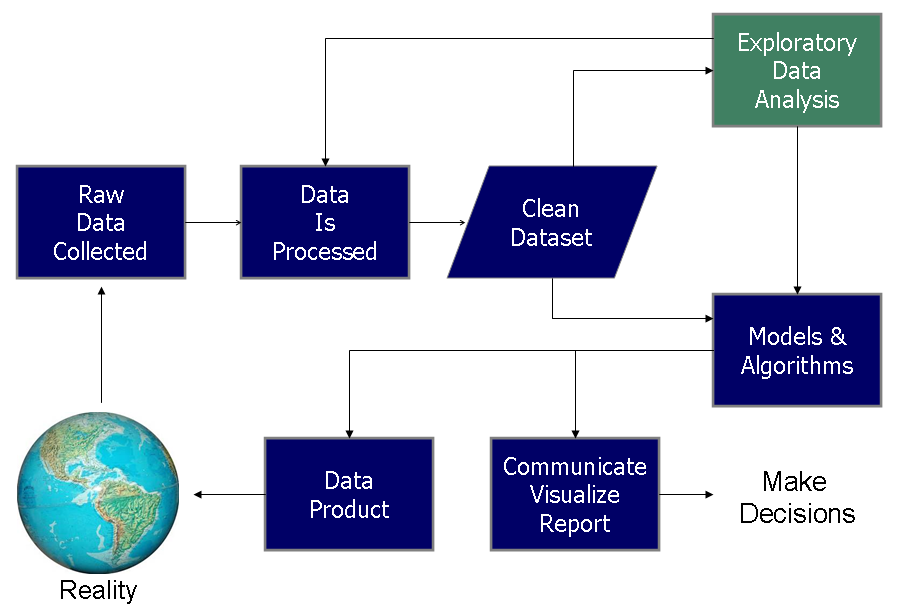
\includegraphics[width=\textwidth]{data_science_process}
	\end{figure}
\end{frame}

%------------------------------------------------

\begin{frame}
	\frametitle{Structure}
	The structure of the notebook will follow the Data Science process seen
	during the exercises.
	\vfill
	\begin{enumerate}
		\define{Data acquisition} from the web, a database, a flat file, etc.
			This includes cleaning the data.
		\vfill
		\define{Data exploration} simple exploratory analysis to describe what
			you got.
		\vfill
		\define{Data exploitation} build and train a Machine Learning algorithm
			based on this data. Any algorithm is considerable, but it has to be
			motivated.
		\vfill
		\define{Evaluation} evaluate the performance, e.g. accuracy, training
			time, etc., of the chosen model. You define the metrics you care
			about!  If you tried multiple algorithms, please report their
			performance and try to explain it.
	\end{enumerate}
\end{frame}

%------------------------------------------------

\begin{frame}
	\frametitle{Practical aspects}
	\begin{itemize}
		\item Please isolate code blocks in functions and put those in a
			separate Python module.
		%\item Maximize the use of external libraries. You should invest time
			%in the problem, not in reinventing the wheel.
		\vfill
		\item Your notebook should be clean and legible.
		\vfill
		\item You can take inspirations from the notebooks seen during the
			exercises.
	\end{itemize}
\end{frame}

%------------------------------------------------

\begin{frame}
	\frametitle{Organization}
	\begin{enumerate}
		\define{Project proposal}
			\begin{itemize}
				\item Single page document explaining what you want to do.
				\item Organize yourselves in groups of one, two or three people.
				\item Deadline: Sunday, November 27, 2016. Upload on Moodle.
				\item Not graded.
			\end{itemize}
		\vfill
		\define{Solution}
			\begin{itemize}
				\item Jupyter notebook with text, math, code, analyzes and
					results.
				\item Deadline: Sunday, January 15, 2017. Upload on Moodle.
				\item The notebook will be posted on the course git repository,
					on GitHub. You can use it for your portfolio!
				\item Graded.
			\end{itemize}
		\vfill
		\define{Presentation}
			\begin{itemize}
				\item Presentation of 15 minutes in front of the class.
				\item Date to be announced, after January 15.
				\item Graded.
			\end{itemize}
	\end{enumerate}
\end{frame}

\end{document}
